\section{Polar}
\label{sec:method}

We target agentic RL tasks where a policy is exercised through an existing harness rather than a custom rollout loop. A task starts from an instruction and a runtime; the harness calls a model endpoint while using tools, editing files, spawning sub-agents, or managing context (compaction, injection, replacement, etc.). After execution, an evaluator assigns an outcome or trace-level reward. The rollout system must preserve the native model interactions as trainer-ready traces: prompt context, sampled assistant tokens, optional behavior-policy log probabilities, loss masks, rewards, and provenance.

\subsection{Architecture}

\polar has two core components: a rollout server and gateway nodes. The rollout service coordinates tasks and global scheduling. Gateway nodes execute sessions, host the model proxy, construct trajectories, and run evaluation. This split keeps durable task management separate from per-session execution and capture.


\begin{figure*}[t]
\centering
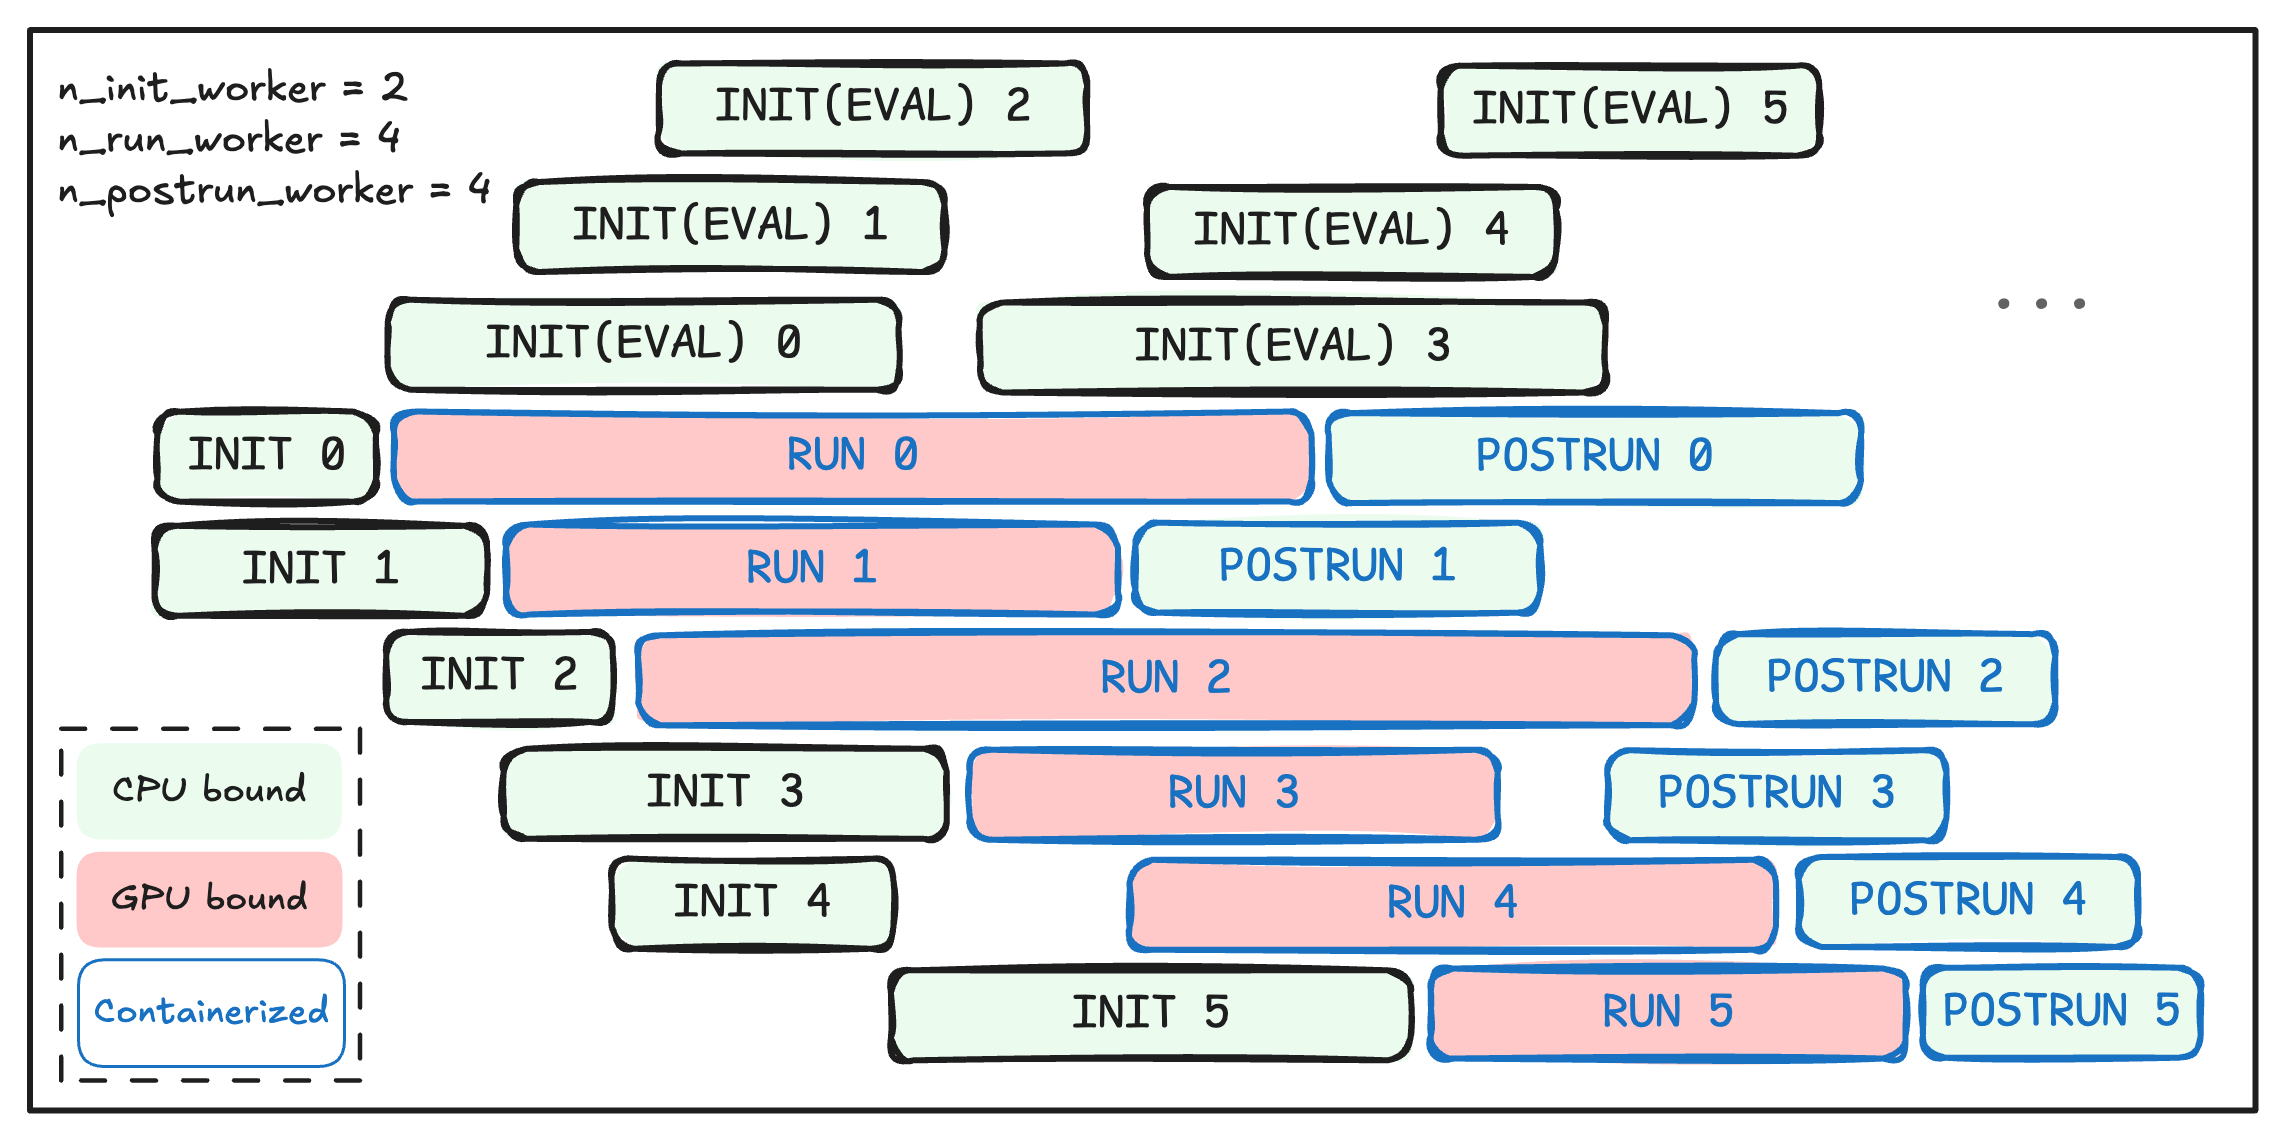
\includegraphics[width=0.86\textwidth]{assets/async_staging.png}
\caption{\textbf{Gateway-level asynchronous staging in \polar.} A gateway separates runtime initialization, ready buffering, harness execution, and post-run trajectory and evaluation work into isolated worker pools. Runtime preparation and evaluator prewarm proceed off the critical path, so CPU-heavy runtime setup and long-tail evaluation do not block active GPU-bound agent run.}
\label{fig:inner_async_staging}
\label{fig:async_staging}
\end{figure*}

\paragraph{Rollout server.}
The rollout service accepts a \texttt{TaskRequest} and expands it into \texttt{num\_samples} independent sessions. A session is the scheduling unit: it has a session ID, task ID, timeout budget, runtime specification, agent specification, trajectory builder, evaluator, and callback URL. The service dispatches sessions to gateway nodes, persists compact terminal results, exposes task status through polling, and accepts gateway callbacks when sessions finish. \Cref{app:task_payload} gives a representative payload.

\paragraph{Gateway node.}
A gateway owns the lifecycle of each session. It starts the runtime, prepares the harness, runs the harness commands, builds trajectories from captured completions, evaluates the output, tears down resources, and returns the result. The same gateway also hosts the proxy endpoint used by the harness for model calls. This co-location keeps completion capture tied to the session registry and avoids a separate trace-collection service.


Training frameworks are independent from \polar servers. And the service boundaries natively supports efficient asynchronous RL at scale. \Cref{fig:outer_async_rl} shows one such example with Slime: a background worker submits \polar tasks, receives task-completion callbacks, converts traces into Slime \texttt{Sample} objects, and applies trajectory-aware reward post-processing.


\subsection{Harness and Proxy Capture}

\polar observes native harnesses by routing their model calls through the gateway proxy. A harness is configured through its normal environment variables or config files so that its model base URL points to the gateway.

For each incoming model request, the gateway performs four steps.

\begin{enumerate}
    \item \textbf{Detect the provider API.} Detection uses the request path and headers to distinguish Anthropic Messages, OpenAI Chat Completions, OpenAI Responses, and Google \texttt{generateContent}-style calls.
    \item \textbf{Normalize the request.} A provider transformer converts roles, content parts, tool definitions, tool choices, stop controls, and generation parameters into the OpenAI Chat Completions shape consumed by local inference servers. The transformer also adds fields needed for training, such as \texttt{logprobs=true}.
    \item \textbf{Capture token-level data.} The gateway forwards the normalized request to the inference servers and stores a completion record containing the request messages, response messages, prompt token IDs, sampled response token IDs, finish reason, and log probabilities from inference backends.
    \item \textbf{Return the provider shape.} The response is transformed back to the schema expected by the harness. For streaming requests, our implementation obtains a non-streaming upstream response and emits a synthetic provider-shaped stream. This simplifies faithful token capture while preserving compatibility with harnesses that expect server-sent events.
\end{enumerate}

The proxy boundary is intentionally below the agent framework. It does not need to understand how the harness plans, manages tools, or decides when to stop. It only needs to preserve API compatibility and record enough information to reconstruct training samples.

\subsubsection{Harness Adapter}

A harness adapter in \polar is small by design. It may install configuration, register MCP servers or skills, write provider settings, and return the shell commands that run the agent. 
A generic \texttt{shell} command harness can be used for wrapped agent execution. We also integrate popular agent harnesses as shortcuts like \texttt{claude\_code}, \texttt{codex}, \texttt{gemini\_cli}, \texttt{qwen\_code}, \texttt{opencode} and \texttt{pi}.

\subsubsection{Runtime Interface}

Runtimes implement a common interface for \texttt{start}, \texttt{stop}, \texttt{exec}, upload, download, and cancellation. Our first release supports Docker and rootless Apptainer for HPC setup. Because gateway code only depends on the runtime interface, a task can change isolation backend without friction.

\subsection{Asynchronous Rollout Staging}

Long-horizon harness rollouts mix several different costs: runtime startup, dependency preparation, harness execution, evaluator setup, test execution, patch application, and teardown. \polar keeps these costs from blocking one another through stage-isolated execution inside each gateway (\cref{fig:async_staging}).

\subsubsection{In-node worker pools.}
Each gateway uses isolated worker pools for \texttt{INIT}, \texttt{RUNNING}, and \texttt{POSTRUN}, plus a bounded \texttt{READY} buffer. \texttt{INIT} starts the runtime and executes prepare actions. \texttt{READY} holds initialized runtimes until a run slot is available. \texttt{RUNNING} executes the harness. \texttt{POSTRUN} builds trajectories, runs evaluators, executes post-run hooks, sends callbacks, and tears down resources. The ready buffer allows CPU-heavy runtime preparation to proceed in the background without blocking GPU-bound agent execution.

% Gateway nodes also report heartbeat metrics to the rollout service, including queue depth, worker capacity, ready-buffer occupancy, and stage inflight counts. The scheduler uses these metrics to avoid unhealthy or draining nodes and to prefer nodes with lower stage pressure.

\subsubsection{Evaluator prewarm and timeouts.}
When an evaluator requests a clean runtime, the gateway begins preparing that runtime during the agent run. Each session also carries one shared deadline; if a harness times out after model calls have been captured, the gateway still enters post-run so partial traces can be recovered with terminal timeout status.

\begin{figure*}[t]
\centering
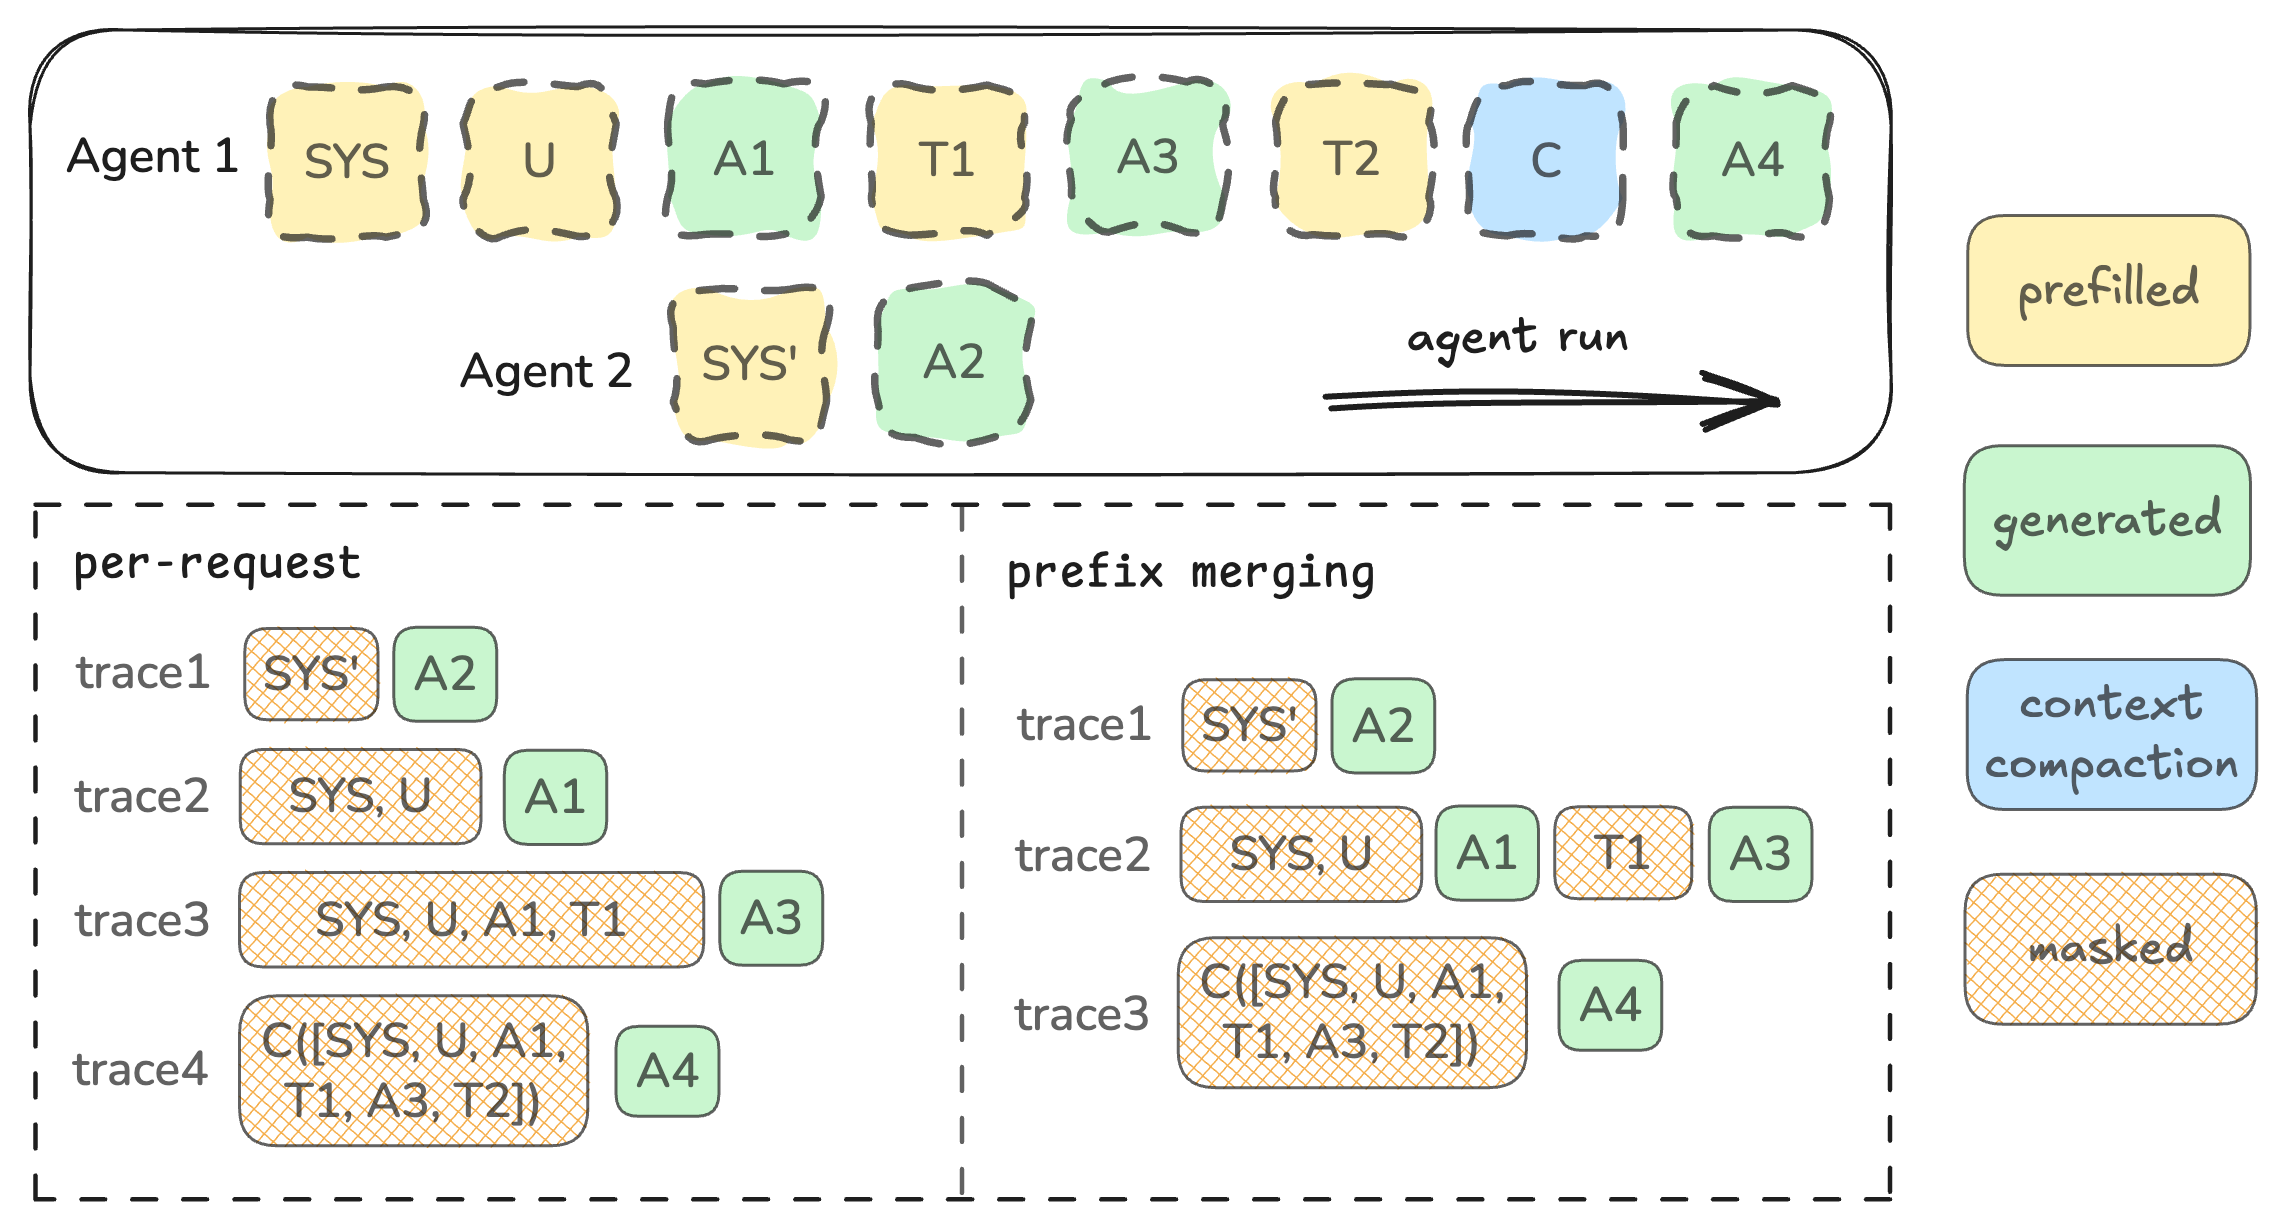
\includegraphics[width=0.76\textwidth]{assets/traj_build.png}
\caption{\textbf{Trajectory reconstruction example.} The visualized session contains a three-turn main agent that undergoes one harness-level context compaction and spawns one subagent. The per-request builder keeps each captured model call as an independent trace. Prefix merging instead recovers append-only conversation chains where valid, while compaction and subagent boundaries naturally form separate chains. Within each merged trace, \polar prefix merging algorithm copies only sampled assistant tokens as trainable tokens and masks canonical interstitial tokens, preserving behavior-policy fidelity while reducing trainer-facing samples.}
\label{fig:trajectory_builder_outputs}
\label{fig:trajectory_builders}
\end{figure*}

\begin{figure*}[t]
\centering
\begin{subfigure}[c]{0.48\textwidth}
\centering
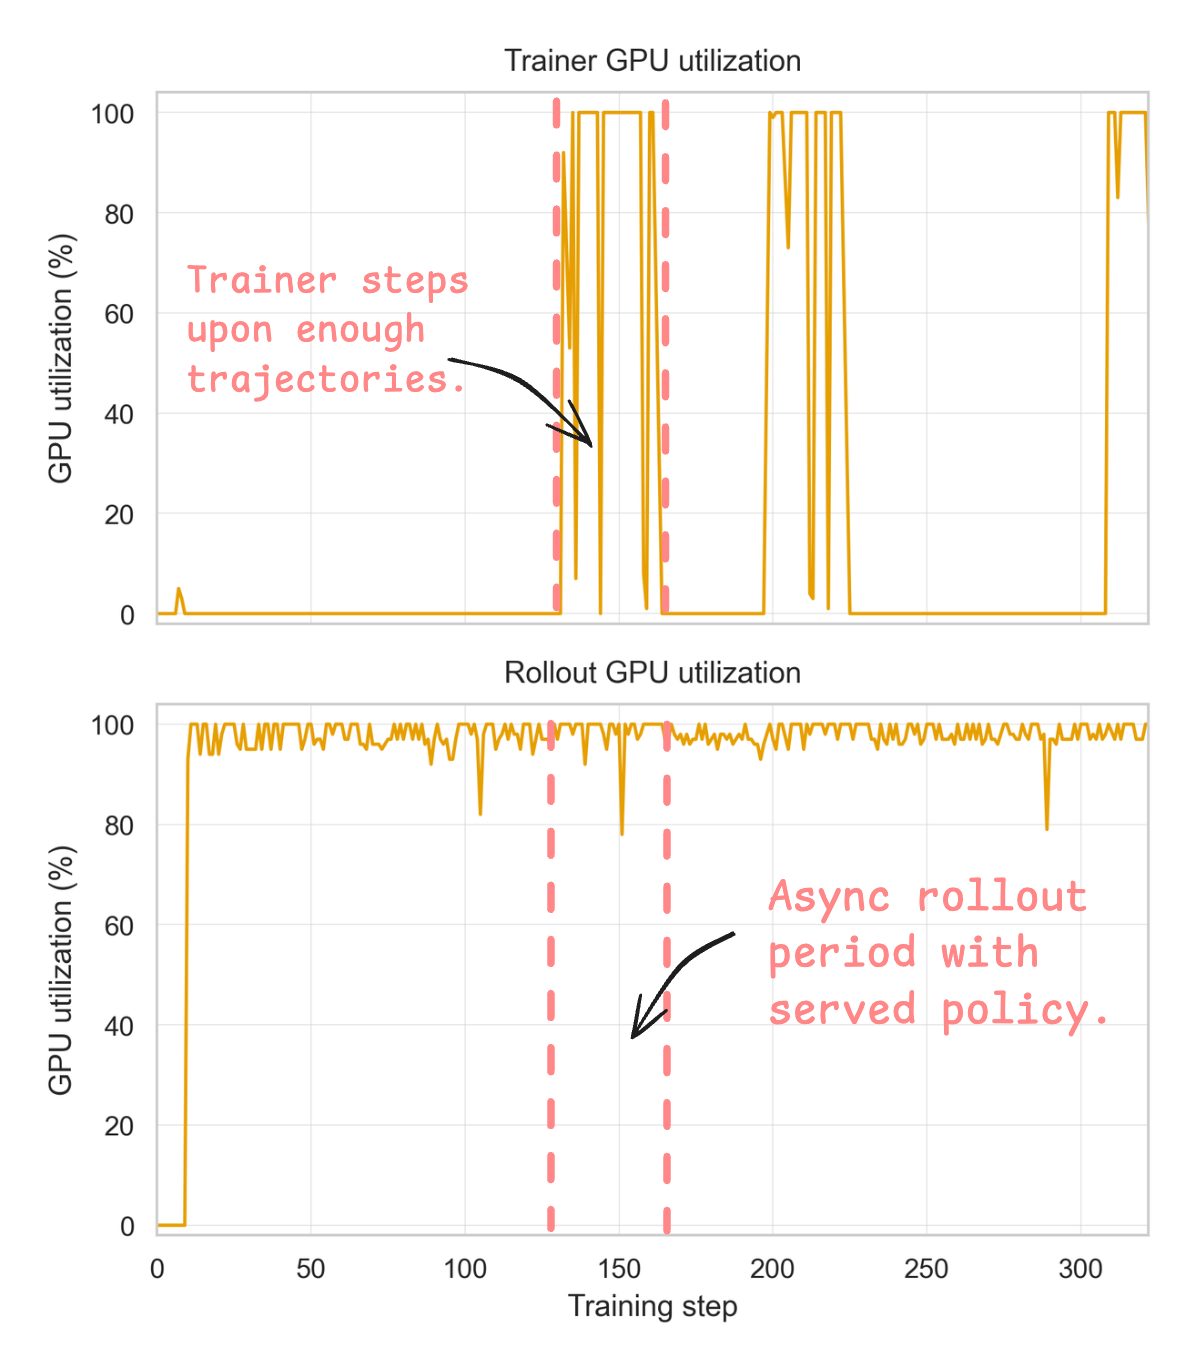
\includegraphics[width=\linewidth]{assets/async_rl_gpu_utilization.png}
\caption{Async RL.}
\label{fig:outer_async_rl}
\end{subfigure}
\hfill
\begin{subfigure}[c]{0.48\textwidth}
\centering
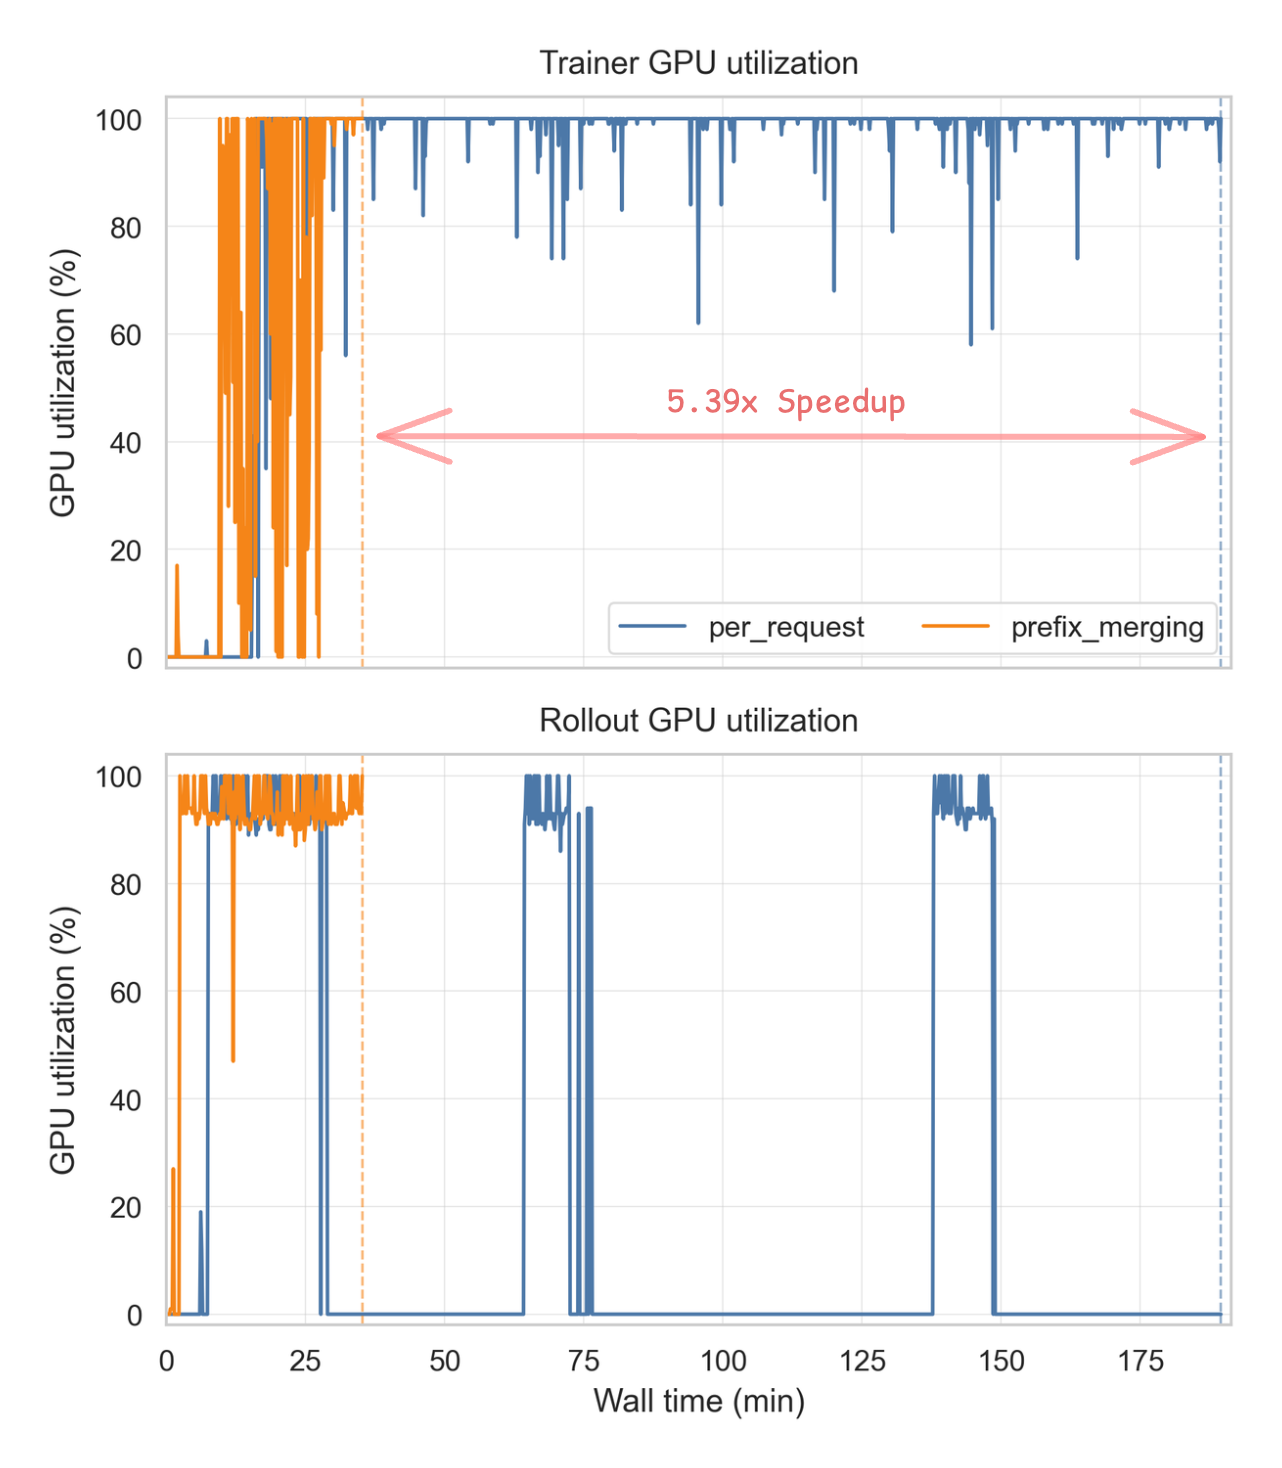
\includegraphics[width=\linewidth]{assets/prefix_merging_vs_per_request_gpu.png}
\caption{GPU utilization with different reconstruction strategies.}
\label{fig:builder_gpu_utilization}
\end{subfigure}
\caption{\textbf{\polar improves GPU utilization across the rollout-training boundary.}
\captiona{} Shows an asynchronous RL pipeline enabled by \polar services. The rollout server keeps inferencing with existing policy, while trainer steps only if receiving batch size of evaluated trajectory groups.
\captionb{} Shows a span of 3 training steps under the same workload and topology, prefix merging emits fewer trainer updates than per-request reconstruction and substantially accelerates the training process.}
\label{fig:rollout_training_utilization}
\end{figure*}

\subsection{Trajectory Reconstruction}

The trajectory builder interface converts an ordered \texttt{CompletionSession} into a \texttt{Trajectory}. A completion session is the stored sequence of proxy-captured model calls for one harness session. A trajectory contains one or more \texttt{Trace} objects, each with prompt token IDs, response token IDs, a loss mask, prompt messages, response messages, tool definitions, log probabilities, reward, and metadata. \Cref{app:trace_example} shows a representative trainer-facing trace.
Custom trajectory strategies can be seamlessly added to the registry, and we provide two strategies, per request and prefix merging, compared in \cref{fig:trajectory_builders}.

\subsubsection{Per Request}

The \texttt{per\_request} builder is the conservative baseline as shown in the bottom left of  \cref{fig:trajectory_builders}: every completion becomes one trace. This is lossless with respect to individual calls, but it can fragment a coherent multi-turn agent session into many short samples. For complex coding harnesses, solving a single coding problem can produce hundreds of such traces, which increases the burden on downstream trainers.


\subsubsection{Token Faithful Prefix Merging}
\label{sec:prefix_merging}

The \texttt{prefix\_merging} builder reconstructs longer traces when parts of a harness session preserve append-only conversation histories as shown in the bottom right of \cref{fig:trajectory_builders}. It does not assume that the whole session is a single conversation. Instead, for a session with completions $C_1,\ldots,C_T$, where completion $C_i$ has prompt token sequence $p_i$, raw sampled response token sequence $a_i$, response log probabilities $\ell_i$, and prompt/response messages $m_i$, \polar partitions the completions into ordered chains
\[
\mathcal{G} = \{G_1,\ldots,G_J\}, \qquad
G_j = (C_{i^j_1}, C_{i^j_2}, \ldots, C_{i^j_{K_j}}),
\]
with $i^j_1 < i^j_2 < \cdots < i^j_{K_j}$. A new completion can join an existing chain only when a normalized message-level grouping key identifies it as a candidate continuation and the strict token-prefix relation holds against the last prompt in that chain. For adjacent completions $C_{i_m}$ and $C_{i_{m+1}}$ inside one chain, this check is
\[
p_{i_{m+1}}[1:|p_{i_m}|] = p_{i_m}.
\]
Thus sub-agents, parallel agent branches, context compaction, prompt rewriting, or independent tool-mediated conversations naturally form additional chains rather than being forced into one global trace.

Merging is then applied independently to each chain. Consider one chain $G=(C_{i_1},\ldots,C_{i_K})$ and write $p_m=p_{i_m}$, $a_m=a_{i_m}$, and $\ell_m=\ell_{i_m}$. The main challenge is that $p_{m+1}$ contains a canonical server rendering of the previous assistant turn plus the interstitial context inserted by the harness before the next generation prompt. The previous assistant body must not be copied from this canonical rendering, because the behavior-policy tokens are the raw sampled tokens $a_m$. Let $e$ denote the end-of-turn token ID. For two adjacent completions in the chain, define the canonical tail
\[
t_m = p_{m+1}[|p_m|+1:].
\]
We locates the first $e$ in $t_m$. If $a_m$ already ends with $e$, the interstitial $u_m$ is the suffix after that $e$; otherwise $u_m$ starts at that $e$ so the assistant turn is still closed before the next prompt context. The token sequence represented by this chain is
\[
z^{(j)} = p_1 \; || \; a_1 \; || \; u_1 \; || \; a_2 \; || \; u_2 \; || \cdots || \; a_K .
\]
The emitted trajectory therefore contains one trace $\tau^{(j)}$ per chain, with the first prompt $p_1$ stored as the trace prompt and the remaining suffix $a_1 || u_1 || \cdots || a_K$ stored as the trace response. The explicit loss mask is one on tokens copied from sampled responses $a_m$ and zero on tokens copied from canonical interstitials $u_m$. Real response log-probability entries are copied for $a_m$ tokens. Interstitial slots receive synthetic log-probability entries so \texttt{response\_logprobs} stays aligned with \texttt{response\_ids}; trainability is controlled by \texttt{loss\_mask}.

This construction gives a simple correctness invariant in every emitted trace:
\begin{center}
    \emph{Every trainable token matches the behavior policy during rollout, and any non-generated tokens are masked out.}
\end{center}

% Boundaries that do not satisfy the append-only token-prefix condition are not merged across; they produce separate traces rather than silent training on retokenized or misaligned assistant text.

\cref{fig:builder_gpu_utilization} compares the GPU utilizations of the 2 strategies above with the same configurations.

\subsection{Evaluation and Reward Propagation}

Evaluators are registry-backed custom strategies that run after trajectory construction. They receive the trajectory, session artifacts, and optionally refreshed runtime context. Built-in evaluators include a session-completion reward, a configurable test-on-output evaluator, and a SWE-Bench/SWE-Gym harness evaluator. An outcome reward can be broadcast to every trace, whereas tasks with process rewards may need per-trace assignment.
The evaluator registry allows straightforward extension to custom rule-based verification, agent-as-judge scoring, and task-specific reward shaping.
